\chapter{Organogenesis: Membangun Tungkai Tetrapoda}\label{ch:b2:limb-organogenesis}

Tiga hari sesudah sebutir telur ayam diletakkan, sebuah benjolan
sebesar kepala jarum muncul pada tiap sisi lembaganya. Empat hari
kemudian ia menjadi sebuah sayap, dengan sebuah humerus, sebuah radius
dan ulna, sebuah pergelangan, dan tiga jari, dalam urutan yang tepat,
dengan panjang yang tepat, dengan otot yang melekat pada tulang yang
tepat. Potonglah rabung kulit menebal pada tepi benjolannya dan
sayapnya berhenti tumbuh; cangkokkan sekerat tepi belakangnya ke
depannya dan ia menumbuhkan enam jari sebagai bayangan cermin. \omterm{def:b2:limb-organogenesis:bud}{Tunas
tungkai} adalah kasus klasik \emph{organogenesis} --- pembangunan sebuah
organ dari sebuah medan sel oleh isyarat yang mengatakan seberapa jauh
ke luar, seberapa jauh ke depan, dan seberapa jauh ke atas letak tiap
selnya --- dan percobaan yang memecahkan sandinya termasuk yang
terjernih dalam biologi. Bab ini mengikuti tunasnya dari pertumbuhan
keluarnya sampai ke rangkanya.

\section{Tunasnya dan ketiga sumbunya}

\begin{definition}[Tunas tungkai]\label{def:b2:limb-organogenesis:bud}
\index{tunas tungkai}\index{rabung ektoderm apikal}%
\index{zona aktivitas pengutuban}
\emph{Tunas tungkai} adalah sebuah pembengkakan \emph{mesoderm lempeng
samping} yang terselubung ektoderm, yang muncul pada kedudukan tetap di
sepanjang sisi tubuhnya (yaitu \emph{medan tungkai}) tempat sandi Hox
sumbu tubuhnya mengizinkannya; mesodermnya akan membuat tulang, rawan,
tendon, dan dermisnya, sedangkan sel yang bermigrasi ke dalamnya dari
somitnya akan membuat ototnya. Tunasnya memiliki tiga sumbu, yang
masing-masing diatur sebuah pusat pengisyaratan.
\emph{Proksimo-distal} (bahu ke ujung jari): \emph{rabung ektoderm
apikal} (AER), yaitu sebuah jalur ektoderm menebal sepanjang ujungnya,
menyekresikan \omterm{prop:b2:limb-organogenesis:aer}{faktor pertumbuhan fibroblas} (FGF) yang menjaga
mesoderm di bawahnya tetap membelah dan tak terdiferensiasi.
\emph{Antero-posterior} (ibu jari ke kelingking): \emph{zona
aktivitas pengutuban} (ZPA), yaitu sebongkah mesoderm pada tepi
belakangnya, menyekresikan morfogen \emph{\omterm{prop:b2:limb-organogenesis:zpa}{Sonic hedgehog}} (Shh).
\emph{Dorso-ventral} (punggung tangan ke telapaknya): ektoderm
punggungnya menyekresikan Wnt7a. Tunas tungkai depan dan belakangnya
tampak serupa dan memakai isyarat yang sama; keduanya berbeda dalam
sebuah faktor transkripsi yang diungkapkan sebelum tunasnya muncul
(Tbx5 pada tungkai depan, Tbx4 pada tungkai belakang), dan itulah
sebabnya sebuah sayap menjadi sayap.
\end{definition}

\begin{omfigure}
\begin{tikzpicture}[every node/.style={font=\scriptsize}, >=stealth]
  % flank
  \fill[omExo!25] (0,-2.2) rectangle (1.2,2.2); \node[rotate=90] at (0.6,0) {dinding tubuh (sisi)};
  % bud outline: paddle
  \draw[thick, fill=omDef!10] (1.2,1.4) .. controls (3.0,1.9) and (5.2,1.6) .. (5.8,0.3) .. controls (5.9,-0.3) and (5.2,-1.6) .. (3.4,-1.7) .. controls (2.4,-1.8) and (1.6,-1.5) .. (1.2,-1.4);
  % AER along the tip
  \draw[line width=3pt, omThm] (5.2,1.3) .. controls (5.9,0.6) and (5.9,-0.6) .. (5.0,-1.4);
  \node[omThm, anchor=west, align=left] at (6.1,0.9) {rabung ektoderm apikal (AER):\\FGF, pertumbuhan proksimo-distal};
  % ZPA posterior
  \draw[thick, omProp, fill=omProp!50] (2.4,-1.1) ellipse (0.55 and 0.4);
  \draw[omProp] (2.4,-1.5) -- (2.4,-2.0);
  \node[omProp, anchor=north, align=center] at (2.6,-2.0) {ZPA (tepi belakang):\\Sonic hedgehog, antero-posterior};
  % dorsal ectoderm
  \draw[line width=2pt, omDef!70!black] (1.4,1.55) .. controls (3.0,2.0) and (5.0,1.7) .. (5.4,1.2);
  \node[omDef!70!black, anchor=south] at (3.4,2.05) {ektoderm punggung: Wnt7a, dorso-ventral};
  % axes
  \draw[->, thick] (1.5,-3.1) -- (5.5,-3.1); \node[below] at (3.5,-3.15) {proksimal $\to$ distal};
  \draw[->, thick] (10.6,-1.6) -- (10.6,1.2); \node[right, align=left] at (10.7,-0.2) {posterior $\to$ anterior\\(kelingking ke ibu jari)};
\end{tikzpicture}

{\small \omterm{def:b2:limb-organogenesis:bud}{Tunas tungkai} anak ayam dilihat dari atas, dengan ketiga pusat
pengisyaratannya: AER di sepanjang ujungnya menggerakkan pertumbuhan
keluarnya, ZPA pada tepi belakangnya memolakan jarinya, dan ektoderm
punggungnya membedakan punggung dari telapaknya.}
\end{omfigure}

\begin{omfigure}
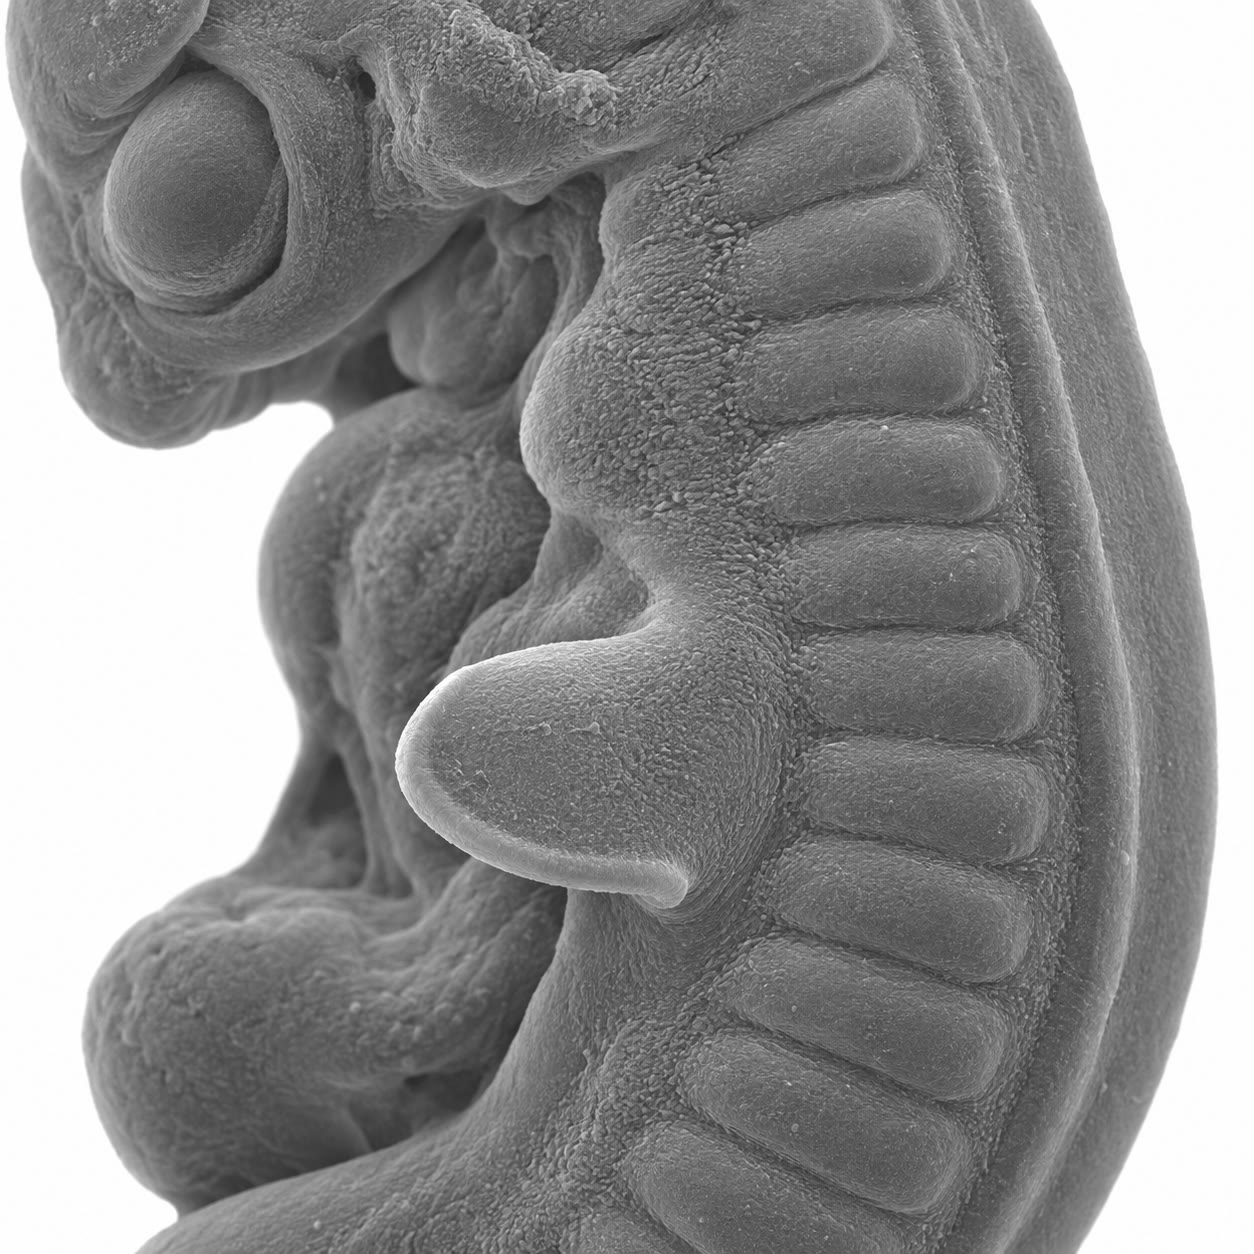
\includegraphics[width=0.42\linewidth]{images/book4/ai/b4-11-limb-bud.jpg}

{\small Sebuah lembaga anak ayam di bawah mikroskop elektron payaran:
deretan somit sepanjang batang tubuhnya dan, pada sisinya, \omterm{def:b2:limb-organogenesis:bud}{tunas
tungkai} berbentuk dayung dengan rabung menebal sepanjang tepinya.}
\end{omfigure}

\section{Pertumbuhan keluar: sumbu proksimo-distal}

\begin{proposition}[Rabung ektoderm apikal]\label{prop:b2:limb-organogenesis:aer}
\index{faktor pertumbuhan fibroblas}\index{zona kemajuan}
AER dibutuhkan bagi pertumbuhan keluarnya dan FGF-nya sudah mencukupi:
mesoderm di bawahnya, yaitu \emph{\omterm{prop:b2:limb-organogenesis:aer}{zona kemajuan}}, membelah kira-kira
tiap dua belas jam, dan sel yang meninggalkan zonanya sembari ujungnya
maju berhenti membelah, memadat, lalu berdiferensiasi. Rangkanya
terbentuk dalam urutan proksimo-distal --- \emph{stilopod} (humerus
atau femur), \emph{zeugopod} (radius dan ulna, tibia dan fibula),
\emph{autopod} (pergelangan dan jari) --- dan tiap ruasnya ditetapkan
bergiliran sembari tunasnya tumbuh, dan ruasnya bersesuaian dengan
daerah bersarang pengungkapan gen Hox (Hoxa/d 9--10 pada stilopodnya,
11 pada zeugopodnya, 13 pada autopodnya). Sebuah \omterm{def:b2:limb-organogenesis:bud}{tunas tungkai} tumbuh
kira-kira sepuluh kali lipat panjangnya dalam empat hari sedangkan
jangkauan isyarat rabungnya tetap beberapa ratus mikrometer yang sama,
sehingga rabungnya memolakan tungkainya bukan sekaligus melainkan
sebagai sebuah muka yang bergerak, seperti sebuah pencetak meletakkan
sehalaman baris demi baris.
\end{proposition}
\begin{proof}[Bukti eksperimental]
Saunders (1948) membuang AER dari tunas sayap anak ayam pada tahap
berturut-turut: dibuang dini, tunasnya hanya memberi sebuah tunggul
humerus; dibuang sehari kemudian, humerus dan lengan bawah tetapi tanpa
tangan; dibuang lebih lambat lagi, sebuah sayap yang nyaris lengkap ---
makin lambat operasinya, makin distal taraf pemenggalannya, sehingga
rabungnya dibutuhkan bagi tiap ruasnya bergiliran. Mencangkokkan sebuah
rabung kedua menghasilkan sebuah pertumbuhan keluar yang kedua; sebuah
manik yang direndam FGF, yang ditaruh pada sebuah tunas yang rabungnya
telah dibuang, memulihkan sebuah tungkai yang lengkap (Niswander,
1993), dan sebuah manik yang ditaruh pada sisi tubuh di antara medan
tungkainya mengimbas sebuah tungkai tambahan. Mencit yang tidak memiliki
FGF rabungnya tidak bertungkai.
\end{proof}

\begin{omfigure}
\begin{tikzpicture}[every node/.style={font=\scriptsize}]
  \foreach \x/\lab/\n in {0/{AER dibuang dini:\\humerus saja}/1, 3.6/{dibuang sehari kemudian:\\humerus, radius, ulna}/2, 7.2/{dibuang lebih lambat lagi:\\sayap nyaris lengkap}/3, 10.8/{utuh:\\sayap lengkap}/4} {
    \begin{scope}[xshift=\x cm]
      \fill[omExo!25] (0,-0.5) rectangle (0.5,2.6);
      % humerus
      \draw[thick, fill=omDef!25, rounded corners=3pt] (0.6,0.9) rectangle (1.7,1.2);
      \ifnum\n>1 \draw[thick, fill=omDef!25, rounded corners=3pt] (1.8,1.05) rectangle (2.7,1.3); \draw[thick, fill=omDef!25, rounded corners=3pt] (1.8,0.75) rectangle (2.7,1.0); \fi
      \ifnum\n>2 \foreach \y in {0.55,0.85,1.15} \draw[thick, fill=omDef!25, rounded corners=2pt] (2.8,\y) rectangle (3.3,\y+0.2); \fi
      \ifnum\n=4 \foreach \y in {0.55,0.85,1.15} \draw[thick, fill=omDef!25, rounded corners=2pt] (3.35,\y) rectangle (3.5,\y+0.2); \fi
      \node[below, align=center] at (1.8,-0.2) {\lab};
    \end{scope}
  }
\end{tikzpicture}

{\small Percobaan Saunders. Makin dini rabungnya dibuang, makin banyak
bagian tungkainya yang hilang, dan selalu dari ujungnya: rabungnya
dibutuhkan bagi tiap ruasnya selagi ruas itu sedang diletakkan.}
\end{omfigure}

\begin{theorem}[Pertumbuhan lewat pembelahan]\label{thm:b2:limb-organogenesis:growth}
Sebuah tunas yang selnya membelah tiap $T$ jam mengalikan cacah selnya
dengan $2^{t/T}$ dalam waktu $t$; empat hari daur dua belas jam memberi
$2^{8} = 256$. Kalau volume tunasnya tumbuh seribu kali lipat dalam
empat hari itu, pembelahannya memasok faktor 256 dan sisa faktor empat
haruslah datang dari pembesaran sel dan matriks yang disekresikan sel
rawan di sekelilingnya. Sebaliknya, sebuah ruas yang memakan satu daur
sel untuk ditetapkan --- kira-kira dua belas jam yang memisahkan taraf
pemenggalan berturut-turut pada percobaan Saunders --- bersesuaian
dengan satu kali pelipatduaan \omterm{prop:b2:limb-organogenesis:aer}{zona kemajuannya}.
\end{theorem}
\begin{proof}
$N(t) = N_0 2^{t/T}$; dengan $t = \qty{96}{h}$ dan $T = \qty{12}{h}$,
$t/T = 8$. Rasio faktor yang dibutuhkan terhadap faktor pembelahannya,
$1000/256 \approx 4$, itulah yang harus disediakan pertumbuhan selain
pembelahannya.
\end{proof}

\section{Jari: sumbu antero-posterior}

\begin{proposition}[Zona aktivitas pengutuban]\label{prop:b2:limb-organogenesis:zpa}
\index{Sonic hedgehog}\index{morfogen!Shh}
ZPA menetapkan jari mana yang terbentuk di mana. Selnya menyekresikan
\omterm{prop:b2:limb-organogenesis:zpa}{Sonic hedgehog}, yang menyebar melintasi tunasnya dari tepi belakangnya,
dan sel mesodermnya membaca kepekatannya --- dan lamanya mereka
terpapar padanya --- sebagai sebuah kedudukan: takaran tertingginya
memberi jari yang paling belakang, takaran yang lebih rendah memberi
jari yang lebih depan, dan di bawah sebuah ambang tidak ada jari sama
sekali. Landaiannya berbentuk eksponensial seperti pada
\cref{ch:b2:vertebrate-development}, dengan panjang peluruhan beberapa
puluh mikrometer, dan ambangnya memotong tunasnya menjadi bakal
jarinya: pada sayap anak ayam, dari belakang ke depan, jari 4, 3, dan 2.
Sebuah sumber isyarat kedua pada tepi depannya menghasilkan sebuah
perangkat kedua sebagai bayangan cermin; sumber yang lebih lemah, atau
paparan yang lebih pendek, hanya menghasilkan jari depan perangkat
tambahannya. Gen yang sama, dalam peran yang sama, memolakan jari tiap
tetrapoda, dan sebuah \omterm{def:b2:genome-diversification:mutation}{mutasi} yang menambahkan sebuah sumber Shh di
depan memberi polidaktili pada kucing, ayam, mencit, dan manusia.
\end{proposition}
\begin{proof}[Bukti eksperimental]
Saunders dan Gasseling (1968) mencangkokkan sebongkah mesoderm tepi
belakang dari satu tunas sayap anak ayam ke tepi depan tunas lainnya:
inangnya menumbuhkan sebuah sayap berjari enam dalam urutan
4-3-2-2-3-4, yaitu sebuah bayangan cermin terhadap tengahnya. Tickle
(1975) menunjukkan bahwa cacah jari tambahannya bergantung pada cacah
sel yang dicangkokkan --- yaitu sebuah takaran. Riddle dan Tabin (1993)
mendapati bahwa jaringan yang dicangkokkan mengungkapkan gen
\emph{\omterm{prop:b2:limb-organogenesis:zpa}{Sonic hedgehog}}, bahwa gennya tidak diungkapkan di tempat lain
mana pun di dalam tunasnya, dan bahwa sel yang direkayasa untuk
mengungkapkannya, yang dicangkokkan di depan, menirukan penggandaan
cerminnya; sebuah manik proteinnya melakukan hal yang sama. Ayam mutan
dengan sebuah bercak Shh salah tempat di depannya memiliki jari depan
tambahan.
\end{proof}

\begin{omfigure}
\begin{tikzpicture}[every node/.style={font=\scriptsize}, >=stealth]
  % normal bud with gradient and digits
  \begin{scope}
    \fill[omExo!25] (0,-0.3) rectangle (0.4,3.3);
    \shade[bottom color=omProp!60, top color=white] (0.4,-0.3) rectangle (3.2,3.3);
    \draw[thick] (0.4,-0.3) rectangle (3.2,3.3);
    \draw[thick, omProp, fill=omProp!70] (0.9,0.1) ellipse (0.45 and 0.35); \node[omProp!80!black, anchor=west] at (1.4,0.1) {ZPA};
    \foreach \y/\d in {0.6/4, 1.5/3, 2.4/2} { \draw[thick, fill=omDef!25, rounded corners=2pt] (3.3,\y-0.12) rectangle (4.2,\y+0.12); \node[right] at (4.25,\y) {jari \d}; }
    \node[below, align=center] at (2.0,-0.5) {tunas normal: Shh dari\\tepi belakangnya, jari 4-3-2};
    \draw[->, thick] (-0.4,0.2) -- (-0.4,3.0); \node[rotate=90] at (-0.7,1.6) {posterior $\to$ anterior};
  \end{scope}
  % grafted bud
  \begin{scope}[xshift=7cm]
    \fill[omExo!25] (0,-0.3) rectangle (0.4,3.3);
    \shade[bottom color=omProp!60, top color=white] (0.4,-0.3) rectangle (3.2,1.5);
    \shade[top color=omProp!60, bottom color=white] (0.4,1.5) rectangle (3.2,3.3);
    \draw[thick] (0.4,-0.3) rectangle (3.2,3.3);
    \draw[thick, omProp, fill=omProp!70] (0.9,0.1) ellipse (0.45 and 0.35);
    \draw[thick, omProp, fill=omProp!70] (0.9,2.9) ellipse (0.45 and 0.35); \node[omProp!80!black, anchor=west] at (1.4,2.9) {ZPA cangkokan};
    \foreach \y/\d in {0.3/4, 0.8/3, 1.3/2, 1.7/2, 2.2/3, 2.7/4} { \draw[thick, fill=omDef!25, rounded corners=2pt] (3.3,\y-0.1) rectangle (4.2,\y+0.1); \node[right] at (4.25,\y) {\d}; }
    \node[below, align=center] at (2.0,-0.5) {ZPA dicangkokkan di depan:\\penggandaan cermin 4-3-2-2-3-4};
  \end{scope}
\end{tikzpicture}

{\small Daerah pengutubannya. Kiri: Shh menyebar dari tepi belakangnya
dan kepekatannya yang menurun menetapkan jari 4, 3, dan 2. Kanan:
sebuah ZPA kedua yang dicangkokkan ke tepi depannya membuat sebuah
landaian kedua dan sebuah perangkat jari bayangan cermin.}
\end{omfigure}

\begin{theorem}[Batas jari dari landaiannya]\label{thm:b2:limb-organogenesis:thresholds}
Dengan Shh berkepekatan $c_0$ pada tepi belakangnya dan panjang
peluruhan $\lambda$, batas wilayah sebuah jari yang ambangnya $T_i$
terletak pada $x_i = \lambda\ln(c_0/T_i)$ dari tepinya. Dengan
$\lambda = \qty{50}{\micro m}$ dan ambang $0.6$, $0.25$, dan $0.08$
dari $c_0$ bagi jari 4, 3, dan 2, wilayahnya adalah $0$--$26$,
$26$--$69$, dan $69$--$126$ mikrometer, dan jaringan di luar
\qty{126}{\micro m} tidak membentuk jari. Melipatduakan sumbernya
menggeser tiap batasnya ke luar sejauh $\lambda\ln 2 = \qty{35}{\micro m}$
--- cukup, pada sebuah tunas beberapa ratus mikrometer, untuk
menambahkan sebuah jari pada tepi depannya; sebuah sumber kedua pada
tepi depannya meletakkan wilayah yang sama secara terbalik.
\end{theorem}
\begin{proof}
Dari $c(x) = c_0 e^{-x/\lambda}$, $c = T_i$ pada $x_i = \lambda
\ln(c_0/T_i)$: $50\ln(1/0.6) = 25.5$, $50\ln 4 = 69$, $50\ln 12.5 =
126$. Mengganti $c_0$ dengan $2c_0$ menambahkan $\lambda\ln 2$ pada tiap
$x_i$.
\end{proof}

\begin{omfigure}
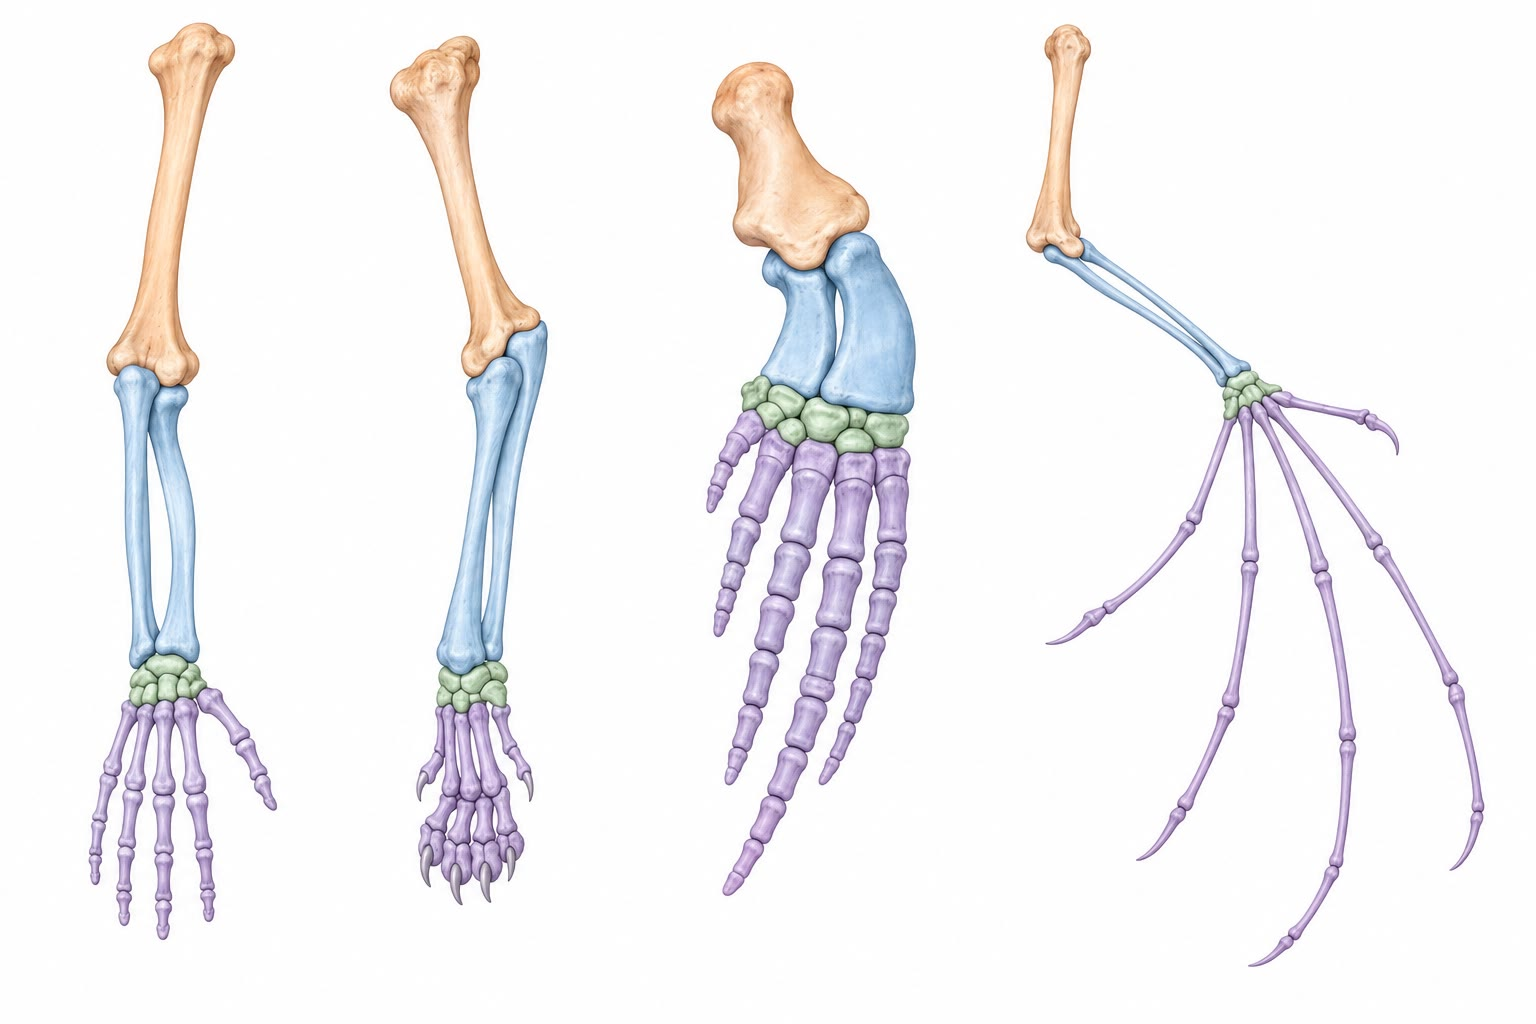
\includegraphics[width=0.66\linewidth]{images/book4/ai/b4-11-tetrapod-limbs.jpg}

{\small Satu rancangan, empat tungkai: tungkai depan manusia, kucing,
paus, dan kelelawar berbagi tulang yang sama dalam urutan yang sama ---
satu stilopod, dua tulang zeugopod, pergelangan, jari --- yang dibangun
pusat pengisyaratan yang sama dan berbeda dalam pertumbuhannya.}
\end{omfigure}

\section{Pemaduan dan pemahatan}

\begin{proposition}[Sumbunya saling berbicara]\label{prop:b2:limb-organogenesis:loop}
\index{gelung umpan balik!perkembangan}
Pusatnya saling mempertahankan: FGF dari rabungnya menjaga ZPA tetap
mengungkapkan Shh, dan Shh, lewat sebuah penyambung di dalam
mesodermnya, menjaga rabungnya tetap mengungkapkan FGF; buanglah salah
satunya dan yang lain memudar dalam sehari. Wnt7a dari ektoderm
punggungnya juga dibutuhkan bagi pengungkapan Shh sepenuhnya, dan ia
menggerakkan nasib punggung mesodermnya (seekor mencit tanpanya
memiliki dua telapak). Saling kebergantungan ini adalah sebuah
\emph{gelung umpan balik positif} yang mengunci ketiga sumbunya
bersama-sama: tungkainya hanya tumbuh di tempat ia sedang dipolakan,
dan hanya dipolakan di tempat ia sedang tumbuh, sehingga sebuah tunas
tidak pernah membuat sebuah tangan tanpa sebuah lengan atau jari yang
keliru macamnya. Ketika pertumbuhan keluarnya selesai, gelungnya
diputus --- mesodermnya berhenti menyambung, Shh-nya berhenti,
rabungnya menyusut --- dan tungkainya berhenti tumbuh pada ukurannya
yang tepat.
\end{proposition}

\begin{proposition}[Dari pola ke tulang]\label{prop:b2:limb-organogenesis:skeleton}
\index{kondrogenesis}\index{apoptosis!antarjari}
Begitu ditetapkan, sel mesoderm yang meninggalkan \omterm{prop:b2:limb-organogenesis:aer}{zona kemajuannya}
\emph{memadat} menjadi tongkat dan lempeng seperti bentuk bakal
tulangnya, berdiferensiasi menjadi sel rawan yang menyekresikan sebuah
matriks yang kaya kolagen dan proteoglikan, lalu meletakkan sebuah
model rawan tiap unsur rangkanya; sendinya terbentuk di tempat
sepanjang pita sel diberi tahu agar tidak menjadi rawan; pembuluh
darahnya menyerbu modelnya dan tulang menggantikan rawannya dari
pusatnya ke luar, sambil meninggalkan lempeng tumbuh pada ujungnya yang
menjaga tulangnya tetap memanjang sampai dewasa
(\emph{pengosifikasian endokondral}). Bakal ototnya dari
somitnya bermigrasi masuk, membelah, lalu melebur menjadi serabut
(\cref{ch:b2:cell-differentiation}) dan melekat lewat tendon yang
dibuat mesoderm tungkainya sendiri. Di antara jari-jarinya, jaringannya
dibuang lewat kematian sel terprogram: sel selaput antarjarinya, yang
diberi tahu sebuah isyarat protein morfogenetik tulang (BMP),
mengaktifkan pemusnahan dirinya sendiri lalu dibersihkan dalam sehari,
dan itulah yang memisahkan jarinya. Seekor bebek mempertahankan
selaputnya karena sebuah penghambat BMP diungkapkan di dalam jaringan
antarjarinya; seekor anak ayam yang diberi penghambat yang sama pada
sebuah manik menumbuhkan kaki berselaput.
\end{proposition}
\begin{proof}[Bukti eksperimental]
Mesoderm antarjari yang dipotong dari tunas kaki anak ayam lalu
dicangkokkan ke tempat lain mati sesuai jadwal --- kematiannya
intrinsik, diputuskan sebelum jaringannya dibuang; jaringan yang sama
dari seekor bebek bertahan hidup. Manik BMP yang ditaruh di antara jari
seekor bebek membuat selaputnya mati; manik penghambat gremlin yang
ditaruh di antara jari seekor anak ayam menyelamatkannya. Seekor mencit
yang tidak memiliki reseptor BMP di tungkainya mempertahankan selaputnya.
\end{proof}

\begin{omfigure}
\begin{tikzpicture}[every node/.style={font=\scriptsize}]
  \foreach \x/\lab in {0/{jari rawan memadat}, 4.2/{sel antarjarinya\\mati (BMP)}, 8.4/{jarinya terpisah;\\tulang menggantikan rawannya}} {
    \begin{scope}[xshift=\x cm]
      \node[below, align=center] at (1.5,-0.3) {\lab};
    \end{scope}
  }
  % stage 1: paddle with rays
  \draw[thick, fill=omDef!8] (0,0) .. controls (0,2.2) and (3,2.2) .. (3,0) -- cycle;
  \foreach \x in {0.6,1.2,1.8,2.4} \draw[thick, fill=omDef!30, rounded corners=2pt] (\x-0.12,0.1) rectangle (\x+0.12,1.5);
  % stage 2: paddle with dying webs
  \begin{scope}[xshift=4.2cm]
    \draw[thick, fill=omDef!8] (0,0) .. controls (0,2.2) and (3,2.2) .. (3,0) -- cycle;
    \foreach \x in {0.6,1.2,1.8,2.4} \draw[thick, fill=omDef!30, rounded corners=2pt] (\x-0.12,0.1) rectangle (\x+0.12,1.5);
    \foreach \x in {0.9,1.5,2.1} \foreach \y in {0.7,1.0,1.3} \fill[omThm] (\x,\y) circle (0.05);
  \end{scope}
  % stage 3: separated digits
  \begin{scope}[xshift=8.4cm]
    \draw[thick, fill=omDef!8] (0,0) -- (0,0.5) -- (0.3,0.5) -- (0.35,1.7) -- (0.85,1.7) -- (0.9,0.5) -- (1.05,0.5) -- (1.1,1.85) -- (1.6,1.85) -- (1.65,0.5) -- (1.8,0.5) -- (1.85,1.7) -- (2.35,1.7) -- (2.4,0.5) -- (2.7,0.5) -- (2.7,0) -- cycle;
    \foreach \x in {0.6,1.35,2.1} \draw[thick, fill=omExo!60, rounded corners=2pt] (\x-0.1,0.1) rectangle (\x+0.1,1.4);
  \end{scope}
\end{tikzpicture}

{\small Memahat tangannya: jari rawan memadat di dalam dayungnya, sel
di antaranya mati (merah), dan jari yang terbebas mengeras menjadi tulang.}
\end{omfigure}

\begin{example}[Tungkai yang sama, ditumbuhkan berbeda]\label{ex:b2:limb-organogenesis:evolution}
Sayap kelelawar adalah sebuah tangan yang jari 2 sampai 5-nya tumbuh
beberapa kali lebih panjang daripada jari mencit --- sebuah penguat
sebuah gen tungkai, yang dipindahkan dari kelelawar ke mencit,
memanjangkan tulang tungkai depan mencitnya --- dan yang jaringan
antarjarinya bertahan hidup, karena selaputnya mengungkapkan penghambat
BMP yang dipakai bebeknya. Sirip paus adalah sebuah tangan dengan ruas
jari tambahan dan tanpa kematian antarjari. Kaki kuda adalah satu jari
tunggal dengan jari lainnya menyusut menjadi bilah. Ular tidak memiliki
tungkai karena sisi tubuhnya tidak pernah mengungkapkan isyarat yang
memulai sebuah tunas. Dan sirip ikan, yang tidak memiliki autopod,
dibangun AER dan ZPA yang sama tetapi menghentikan program Hox-nya
sebelum fase akhir yang membuat jari; fosil \emph{Tiktaalik} (berumur
375 juta tahun) memperlihatkan pergelangan yang muncul di dalam sebuah
sirip. Evolusi tungkai sebagian besar adalah pemodulasian sebuah program
yang lestari --- berapa lama tiap fasenya berjalan, seberapa jauh tiap
isyaratnya menjangkau, sel mana yang mati.
\end{example}

\section{Latihan}

\begin{exercise}[$\star$]\label{exo:b2:limb-organogenesis:1}
Sebutkan ketiga sumbu \omterm{def:b2:limb-organogenesis:bud}{tunas tungkainya} dan, bagi masing-masingnya,
pusat pengisyaratannya, kedudukannya, dan isyaratnya.
\end{exercise}

\begin{exercise}[$\star$]\label{exo:b2:limb-organogenesis:2}
Berikan ketiga ruas rangka tungkainya dan tulang tiap ruasnya pada
lengan dan kaki manusia. Gen Hox mana yang menandainya?
\end{exercise}

\begin{exercise}[$\star$]\label{exo:b2:limb-organogenesis:3}
Daftarkan, menurut urutannya, langkah dari sebercak mesoderm lempeng
samping sampai ke sebuah jari beserta tulang, sendi, dan ototnya.
\end{exercise}

\begin{exercise}[$\star$]\label{exo:b2:limb-organogenesis:4}
Tungkainya tampak seperti apa kalau AER-nya dibuang (a) begitu tunasnya
muncul, (b) sesudah lengan bawahnya ditetapkan, (c) sama sekali tidak
dibuang melainkan digantikan sebuah manik FGF?
\end{exercise}

\begin{exercise}[$\star\star$]\label{exo:b2:limb-organogenesis:5}
Dengan $\lambda = \qty{40}{\micro m}$ dan ambang $0.5$, $0.2$, dan
$0.05$ dari kepekatan sumbernya bagi jari 4, 3, dan 2, hitunglah ketiga
batasnya dan lebar tiap wilayah jarinya.
\end{exercise}

\begin{exercise}[$\star\star$]\label{exo:b2:limb-organogenesis:6}
Ramalkanlah pola jari sebuah sayap anak ayam sesudah (a) sebuah ZPA
penuh dicangkokkan ke tepi depannya, (b) sebuah cangkokan berisi
seperempat cacah sel ZPA-nya, (c) sebuah manik Shh pada tepi depannya
yang dibuang sesudah paparan yang pendek. Jelaskan masing-masingnya
dari segi takaran dan waktunya.
\end{exercise}

\begin{exercise}[$\star\star$]\label{exo:b2:limb-organogenesis:7}
Sebuah \omterm{def:b2:limb-organogenesis:bud}{tunas tungkai} anak ayam memiliki \num{5000} sel ketika rabungnya
terbentuk dan selnya membelah tiap \qty{12}{h}. Berapa selnya sesudah
empat hari? Kalau tungkainya pada tahap itu memiliki $4\times 10^{6}$
sel, apa yang pastilah benar tentang daur selnya atau tentang kematian
selnya?
\end{exercise}

\begin{exercise}[$\star\star$]\label{exo:b2:limb-organogenesis:8}
Jelaskan mengapa anak ayam berjari kaki bebas dan bebek berkaki
selaput, serta apa yang dikerjakan sebuah manik penghambat BMP di
antara jari kaki sebuah lembaga anak ayam. Apa yang dikatakan waktu
intrinsik kematian antarjarinya (ia terjadi sesuai jadwal pada sebuah
cangkokan) tentang bagaimana selnya diperintah?
\end{exercise}

\begin{exercise}[$\star\star$]\label{exo:b2:limb-organogenesis:9}
Seekor mencit tidak memiliki Hoxa13 maupun Hoxd13; mencit lain tidak
memiliki Hoxa11 maupun Hoxd11. Ramalkanlah rangka tungkai depan
masing-masingnya lalu katakan apa yang ditunjukkan hasilnya tentang
hubungan antara daerah Hox dan ruasnya.
\end{exercise}

\begin{exercise}[$\star\star\star$]\label{exo:b2:limb-organogenesis:10}
Jelaskan umpan balik positif antara AER dan ZPA-nya, mengapa ia
membuat tungkainya tegar, dan apa yang akan terjadi pada sebuah tunas
yang Shh-nya tidak dapat mempertahankan FGF-nya. Pertentangkan dengan
umpan balik positif persalinan pada \cref{ch:b2:mammal-reproduction}:
apa yang mengakhiri tiap gelungnya?
\end{exercise}

\begin{exercise}[$\star\star\star$]\label{exo:b2:limb-organogenesis:11}
Jari ketiga seekor kelelawar delapan kali lebih panjang daripada jari
seekor mencit relatif terhadap ukuran tubuhnya. Kalau rawan jarinya
memanjang secara eksponensial dengan laju $r$ tiap hari selama sebuah
jendela pertumbuhan, dan jendela kelelawarnya empat hari lebih panjang
daripada jendela mencitnya, $r$ berapa yang dibutuhkan? Berikan dua
perubahan perkembangan (satu dalam pertumbuhannya, satu dalam kematian
selnya) yang membuat sebuah sayap dari sebuah tangan.
\end{exercise}

\begin{exercise}[$\star\star\star$]\label{exo:b2:limb-organogenesis:12}
\omterm{prop:b2:limb-organogenesis:zpa}{Sonic hedgehog} memolakan \omterm{prop:b2:vertebrate-development:neurulation}{tabung saraf} dari lempeng lantainya
(\cref{ch:b2:vertebrate-development}) dan memolakan jari dari ZPA-nya.
Bahaslah mengapa evolusi memakai ulang segelintir isyarat bagi banyak
pekerjaan, bagaimana molekul yang sama dapat berarti berbeda di dalam
jaringan yang berbeda, dan apa yang disiratkannya bagi pengaruh sebuah
\omterm{def:b2:genome-diversification:mutation}{mutasi} pada gen semacam itu.
\end{exercise}

\section{Soal: Sebuah Sayap yang Dibangun dalam Sepekan}

\begin{problem}[{Soal akhir pekan --- sayap anak ayam diikuti dari
tunas sampai rangka: pertumbuhannya lewat pembelahan, pembuangan
rabung Saunders diwaktui, landaian Shh-nya dihitung dan penggandaannya
diramalkan, selaputnya dipahat dan sayapnya dibandingkan dengan sayap
kelelawar, berakhir pada cacah pelipatduaannya, batas jarinya, dan
lebar yang dibutuhkan sebuah tunas bagi sebuah penggandaan cermin}]
\label{pb:b2:limb-organogenesis:1}
Sebuah tunas sayap anak ayam muncul pada 3 hari pengeraman dengan
\num{2000} sel mesoderm dan panjang \qty{0.4}{mm}; pada 7 hari sayapnya
sepanjang \qty{4}{mm} dan volumenya \num{1000} kali volume tunasnya.
Sel \omterm{prop:b2:limb-organogenesis:aer}{zona kemajuannya} membelah tiap \qty{12}{h}. Pembuangan rabungnya:
pada 3,0 hari tungkainya sebuah tunggul; pada 3,5 hari hanya sebuah
humerus; pada 4,0 hari humerus, radius, dan ulna; pada 4,5 hari sebuah
sayap yang hanya kekurangan ujung jarinya. Shh: $D = \qty{1e-12}{m^2/s}$, waktu paruh \qty{29}{min}; ambang $0.6$, $0.25$,
$0.08$ dari $c_0$ bagi jari 4, 3, 2. Lebar tunasnya (belakang ke depan)
\qty{600}{\micro m}. Selaput antarjarinya: tiga daerah berukuran
\qty{300}{\micro m}$\times$\qty{300}{\micro m}$\times$\qty{200}{\micro m}, dengan sel
berukuran \qty{1000}{\micro m^3}, yang dibersihkan dalam \qty{24}{h}.

\medskip
\noindent\textbf{Bagian I --- Pertumbuhannya.}
\begin{enumerate}
  \item Berapa kali pelipatduaan yang terjadi dalam empat hari? Berapa
        sel yang diberikannya dari \num{2000}?
  \item Bandingkan dengan kenaikan volume seribu kali lipatnya: faktor
        berapa yang harus disediakan pembesaran sel dan matriksnya?
  \item Dengan faktor berapa panjangnya tumbuh? Kalau tunasnya tumbuh
        sebagai sebuah silinder berjari-jari tetap, faktor volume
        berapa yang akan diperolehnya, dan apa yang dikatakan
        perbedaannya tentang bentuknya?
  \item FGF rabungnya menjangkau \qty{300}{\micro m} ke dalam
        mesodermnya. Berapa bagian tunasnya yang berada di bawah
        pengaruhnya pada 3 hari dan pada 7 hari?
  \item Jelaskan mengapa sebuah isyarat berjangkauan tetap di dalam
        sebuah organ yang tumbuh menghasilkan sebuah urutan
        proksimo-distal.
  \item Sebuah sel meninggalkan \omterm{prop:b2:limb-organogenesis:aer}{zona kemajuannya} pada 4 hari. Ruas mana
        yang dimasukinya?
\end{enumerate}

\medskip
\noindent\textbf{Bagian II --- Mewaktui ruasnya.}
\begin{enumerate}[resume]
  \item Dari deret pembuangannya, berikan waktu saat tiap ruasnya
        (stilopod, zeugopod, autopod) telah ditetapkan.
  \item Berapa daur sel yang memisahkan penetapan ruas yang
        berturut-turut?
  \item Jelaskan hasilnya dari segi \omterm{prop:b2:limb-organogenesis:aer}{zona kemajuan} dan daerah
        Hox-nya.
  \item Sebuah manik FGF ditaruh pada sebuah tunas yang rabungnya
        dibuang pada 3,5 hari. Ramalkanlah tungkainya.
  \item Sebuah rabung kedua dicangkokkan ke permukaan punggung sebuah
        tunas yang utuh pada 3,5 hari. Ramalkanlah.
  \item Mengapa tunasnya berhenti tumbuh pada 7 hari alih-alih terus
        tumbuh tanpa batas?
\end{enumerate}

\medskip
\noindent\textbf{Bagian III --- Landaiannya.}
\begin{enumerate}[resume]
  \item Hitunglah $k$ dan $\lambda$ bagi Shh-nya.
  \item Hitunglah ketiga batas jarinya dan lebar wilayahnya.
  \item Seberapa lebar daerah depan yang tidak membentuk jari pada
        sebuah tunas \qty{600}{\micro m}?
  \item Sebuah \omterm{def:b2:genome-diversification:mutation}{mutasi} melipatduakan keluaran Shh-nya. Hitunglah kembali
        batasnya lalu katakan apakah sebuah jari tambahan terbentuk dan
        jari yang mana.
  \item Sebuah ZPA dicangkokkan ke tepi depannya. Lebar tunas minimal
        berapa yang memungkinkan sebuah perangkat cermin lengkap
        4-3-2-2-3-4 tanpa tindihan kedua wilayah jari 2-nya? Apakah
        tunas anak ayamnya cukup lebar?
  \item Ramalkanlah polanya kalau tunasnya hanya selebar
        \qty{200}{\micro m}.
  \item Mengapa sebuah cangkokan berisi seperempat ZPA-nya hanya
        memberi 2-2-3-4?
\end{enumerate}

\medskip
\noindent\textbf{Bagian IV --- Pemahatan dan evolusinya.}
\begin{enumerate}[resume]
  \item Hitunglah cacah sel di dalam ketiga selaputnya dan laju
        kematian selnya selama pembersihannya, dalam sel tiap sekon.
  \item Sel antarjari seekor bebek mengungkapkan sebuah penghambat BMP.
        Ramalkanlah pengaruh sebuah manik BMP di dalam selaput bebeknya
        dan pengaruh penghambatnya di dalam selaput anak ayamnya.
  \item Rawan jari seekor kelelawar tumbuh empat hari tambahan pada
        laju eksponensial \qty{0.5}{d^{-1}}. Dengan faktor berapa ia
        lebih panjang daripada rawan anak ayamnya? Sebutkan perubahan
        kedua yang membuat selaput sayapnya.
  \item Sebuah tunas sirip ikan memiliki sebuah AER dan sebuah ZPA
        tetapi tidak berjari. Apa yang hilang, dan apa yang ditunjukkan
        \emph{Tiktaalik}?
  \item Kalau sel selaputnya sebagai gantinya dihasilkan lewat
        pembelahan dari \num{1000} pendiri pada \qty{12}{h} tiap
        daurnya, berapa lama membuatnya? Bandingkan dengan sehari yang
        dibutuhkan untuk membuangnya.
  \item Nyatakan hasilnya: cacah pelipatduaan dalam empat hari, ketiga
        batas jarinya, dan lebar minimal bagi sebuah penggandaan cermin.
\end{enumerate}
\end{problem}
